%----------------------------------------------------------------------------------------
%    PACKAGES AND THEMES
%----------------------------------------------------------------------------------------

\documentclass[aspectratio=169,xcolor=dvipsnames]{beamer}
\usetheme{SimplePlus}

\usepackage{hyperref}
\usepackage{graphicx} % Allows including images
\usepackage{booktabs} % Allows the use of \toprule, \midrule and \bottomrule in tables

\usepackage[caption=false]{subfig}

\usepackage{tikz}
\usetikzlibrary{positioning}

\usepackage{pgfplots}
\usepgfplotslibrary{groupplots}
\pgfplotsset{compat=1.18}

\usepackage{xspace}
\usepackage{blkarray}

\newcommand{\backupbegin}{
    \newcounter{finalframe}
    \setcounter{finalframe}{\value{framenumber}}
}
\newcommand{\backupend}{
    \setcounter{framenumber}{\value{finalframe}}
}

\newcommand{\modelministral}{Ministral-8B\xspace}
\newcommand{\modelalpaca}{Alpaca-7B\xspace}
\newcommand{\modeldeepseek}{R1-Distill-8B\xspace}

%----------------------------------------------------------------------------------------
%    TITLE PAGE
%----------------------------------------------------------------------------------------

\title{Knowledge Graph Completion}
\subtitle{}

\author{Eddie Groh \and Mochamad Ardiansyah Nurgaha \and Sriraam Appakutti Palani \and William Liaw}

\institute[Team: AWESome]
{
    Language Models and Structured Data\\
}
\date{\today}

%----------------------------------------------------------------------------------------
%    PRESENTATION SLIDES
%----------------------------------------------------------------------------------------

\begin{document}

\begin{frame}
    % Print the title page as the first slide
    \titlepage
\end{frame}

% \begin{frame}{Overview}
%     \tableofcontents
% \end{frame}

%------------------------------------------------


\begin{frame}{Problem Statement}
    \textbf{\textit{KGC infers missing facts in a knowledge graph.}}\\
    \vspace{0.3cm}
    \textbf{\textit{1. Link Prediction}} % - Predict a missing entity in (h, r, ?) or (?, r, t).
    \begin{itemize}
        \item  Ranking of candidate entities.
    \end{itemize}

    \begin{center}
        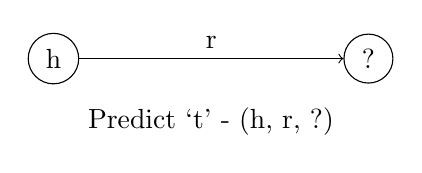
\begin{tikzpicture}
            \node[draw, circle] (h) at (0,0) {h};
            \node[draw, circle] (t) at (4,0) {?};
            \draw[->] (h) -- node[above] {r} (t);
            \node[below] at (2,-0.5) {Predict `t' - (h, r, ?)};
        \end{tikzpicture}
    \end{center}
    %\vspace{-0.3cm}
    %\small{Fig: Predicting missing tail entity for a given head and relation.}\\

    \textit{\textbf{2. Triple Classification}} % - Verify the validity of a given triple (h, r, t)
    \begin{itemize}
        \item Provide a binary classification: \textbf{valid} or \textbf{invalid}.
    \end{itemize}

    \begin{center}
        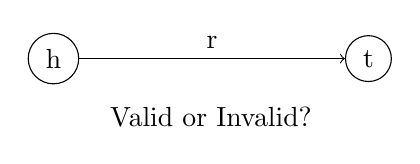
\begin{tikzpicture}
            \node[draw, circle] (h2) at (0,0) {h};
            \node[draw, circle] (t2) at (4,0) {t};
            \draw[->] (h2) -- node[above] {r} (t2);
            \node[below] at (2,-0.5) {Valid or Invalid?};
        \end{tikzpicture}
    \end{center}
    %\small{Fig: Checking if a given relation between two entities is valid.}
\end{frame}


\begin{frame}{Background - LLM-Based Approaches}

    \vspace{0.2cm}
    \textbf{\textit{1. Purely Prompt-Based Methods}}
    \begin{itemize}
        \item Structured retrieval and in-context learning.
        \item \textbf{KICGPT} – triple-based retriever and Knowledge Prompts.
        %\item No need to fine-tune the LLM.
    \end{itemize}

    \textbf{\textit{2. Fine-Tuning-Based Methods}}
    \begin{itemize}
        \item KG structure into LLM parameters.
        \item \textbf{KoPA} - Knowledge Prefix Adapter.
        % \item Provides better \textbf{alignment} with KG schemas.
    \end{itemize}

    \vspace{0.3cm}
    \begin{center}
        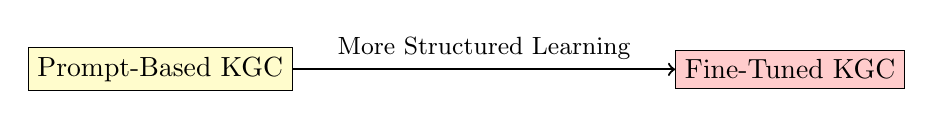
\begin{tikzpicture}
            \node[draw, rectangle, fill=yellow!20] (prompt) at (0,0) {Prompt-Based KGC};
            \node[draw, rectangle, fill=red!20] (fine) at (8,0) {Fine-Tuned KGC};
            \draw[->, thick] (prompt) -- node[above] {\small More Structured Learning} (fine);
        \end{tikzpicture}
    \end{center}

\end{frame}

%------------------------------------------------
\begin{frame}{KICGPT: Retrieval-Augmented Prompting}
    Idea: \textbf{ranking of entities} and \textbf{in-context learning} (ICL)
    % \begin{itemize}
    %     \item Retrieve candidate entities from the KG.
    %     \item Generate Knowledge Prompts for ICL.
    %     \item Perform reranking using a LLM.
    % \end{itemize}
    \begin{center}
        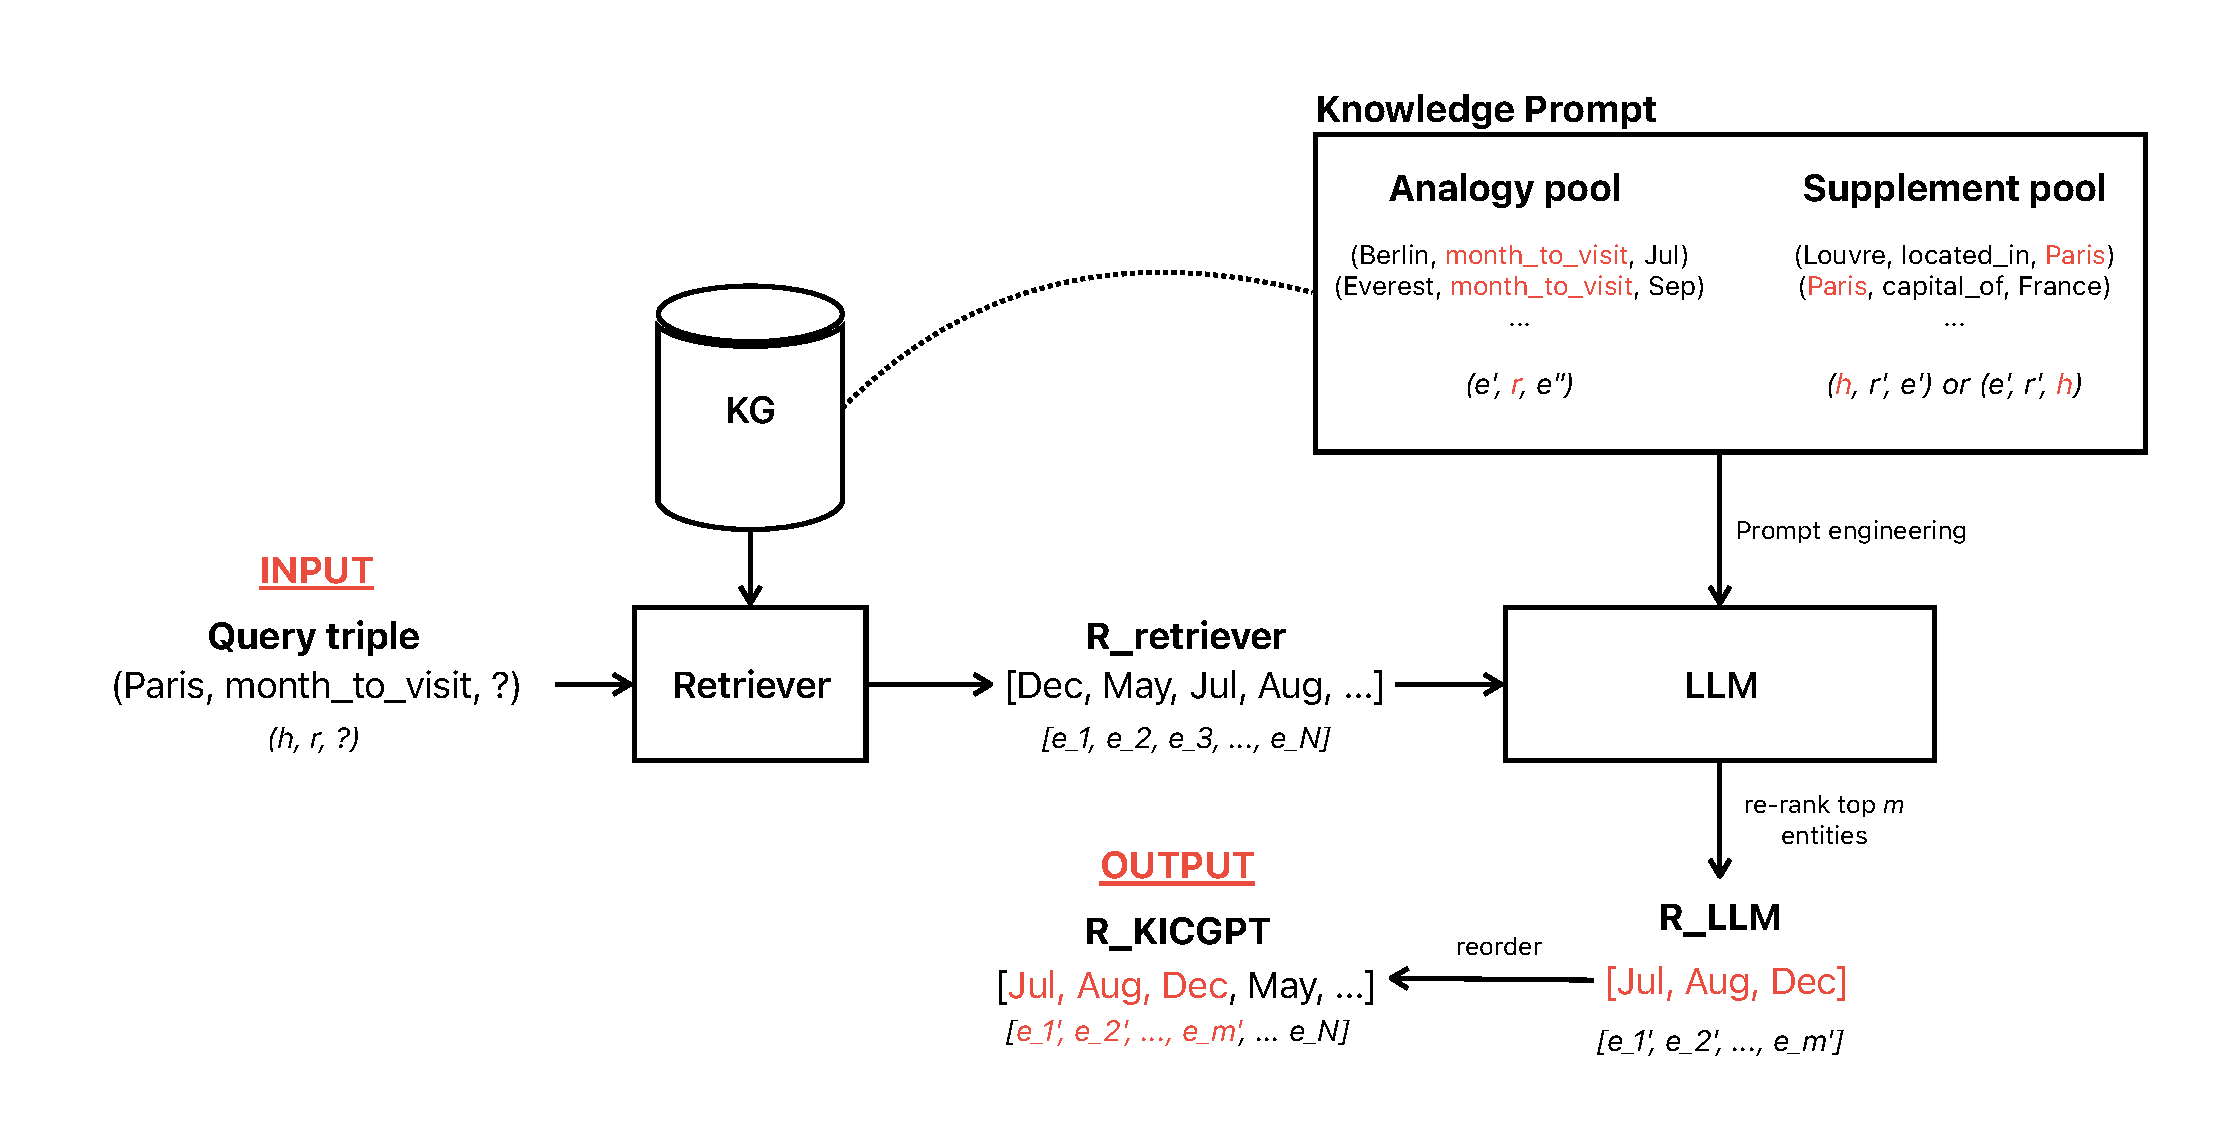
\includegraphics[width=1.02\linewidth]{images/KICGPT}
        % \caption{KICGPT Architecture}
    \end{center}
\end{frame}

% talk about the following:
% - abbreviation of KICGPT
% - KICGPT main ideas: ranking of entities, ICL
% - flow of KICGPT with example

\begin{frame}{KoPA: Fine-Tuning-Based Triple Classification}
    Idea: integrate \textbf{KG structure as prefix} and \textbf{fine-tuning}
    % \begin{itemize}
    %     \item Pre-training: extract structural information of entities and relations.
    %     \item Uses Knowledge Prefix Adapter (KPA) to integrate KG structural embeddings $\rightarrow$ help LLM reasoning.
    %     % \item Embeddings guide LLM reasoning.
    %     \item Fine-tuned LLM predicts validity of triples.
    % \end{itemize}
    \begin{center}
        \centering
        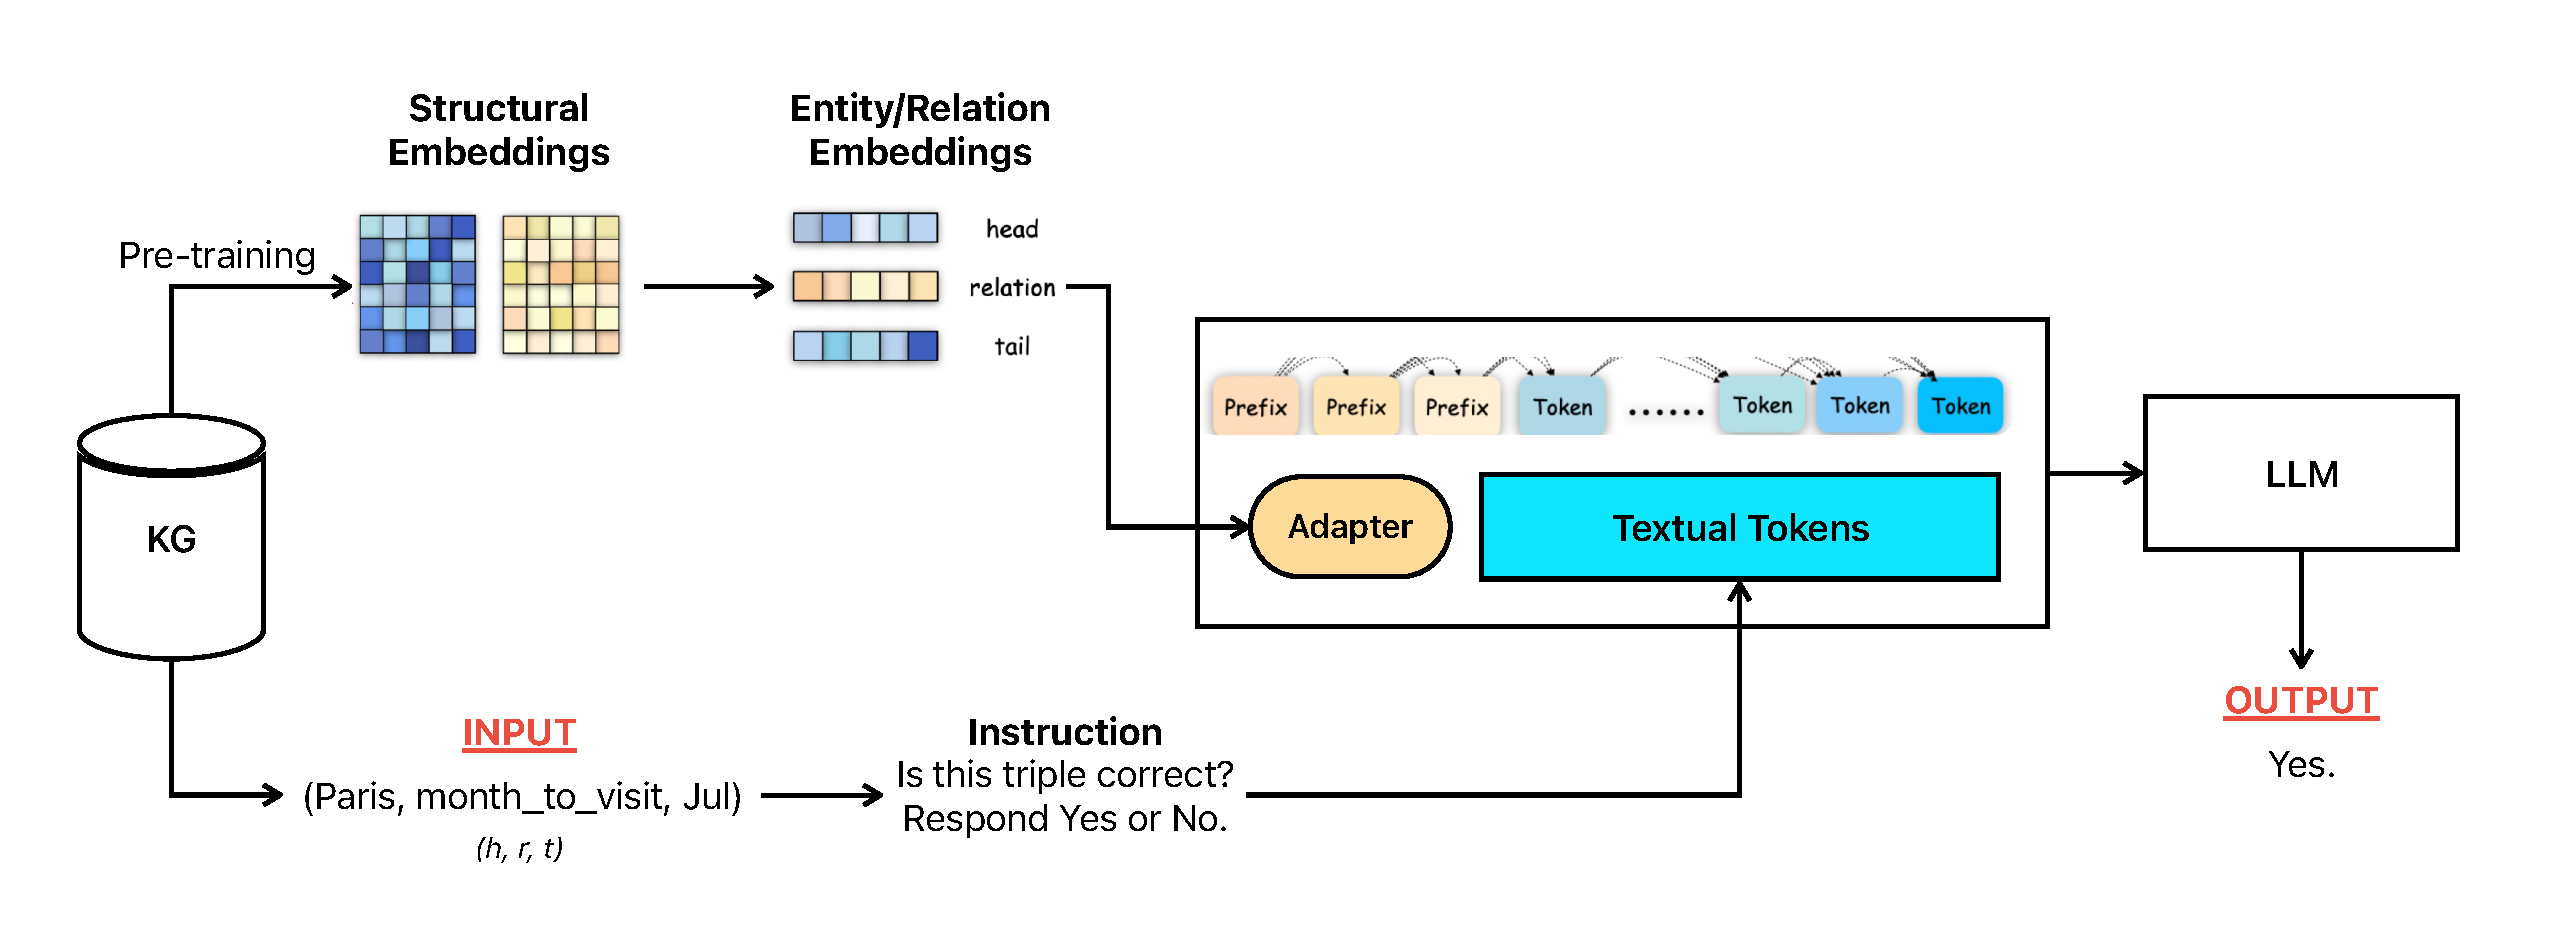
\includegraphics[width=1\linewidth]{images/KoPA}
        % \caption{KoPA Architecture}
    \end{center}
\end{frame}

%------------------------------------------------

% Fine-tuning two models:
% Alpaca: Used in original paper, optimized for instruction following
% Deepseek: Distill from

\begin{frame}{KICGPT: Prompting \hfill KoPA: Fine-tuning\hspace{20mm}}
    \begin{columns}[c]
        \centering
        \column{.49\textwidth}
        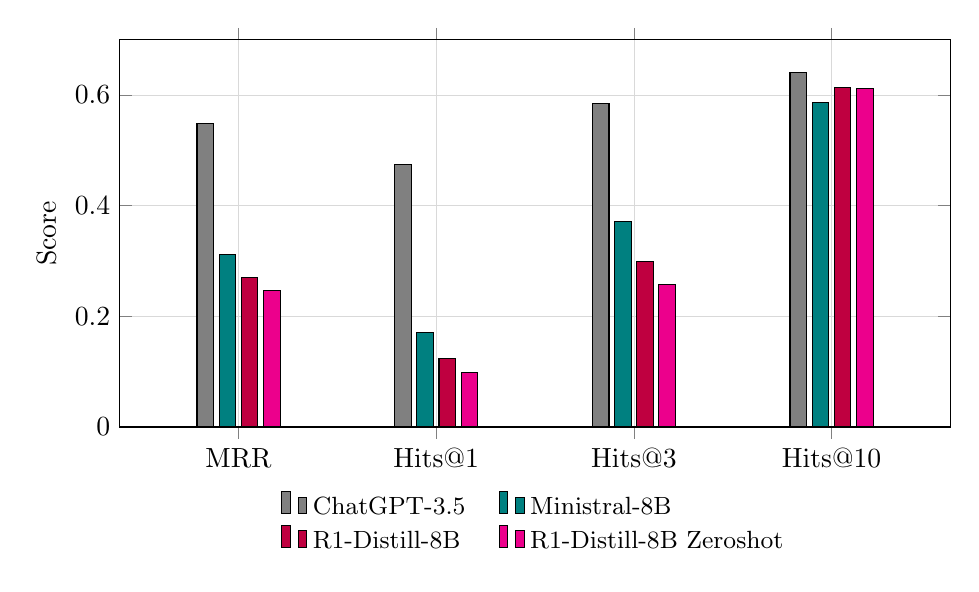
\begin{tikzpicture}
            \begin{axis}[
                ybar, bar width=6pt,
                symbolic x coords={MRR, Hits@1, Hits@3, Hits@10},
                xtick=data, ymin=0, ymax=0.7, ylabel={Score}, width=\textwidth, height=6.5cm, grid=both,
                major grid style={line width=.2pt, draw=gray!30},
                minor grid style={draw=gray!10},
                enlarge x limits=0.2,
            % Legend placed below with spacing:
                legend style={
                    at={(0.5,-0.15)}, anchor=north,
                    /tikz/every even column/.append style={column sep=10pt},
                    legend columns=2, draw=none, fill=none, font=\small,
                    nodes={anchor=west}
                }]
                % Bars
                \addplot[fill=gray]   coordinates {(MRR,0.549)  (Hits@1,0.474)  (Hits@3,0.585)  (Hits@10,0.641)};
                \addlegendentry{ChatGPT-3.5}
                \addplot[fill=teal]   coordinates {(MRR,0.3112) (Hits@1,0.1707) (Hits@3,0.3711) (Hits@10,0.5862)};
                \addlegendentry{\modelministral}
                \addplot[fill=purple] coordinates {(MRR,0.2700) (Hits@1,0.1233) (Hits@3,0.2994) (Hits@10,0.6145)};
                \addlegendentry{\modeldeepseek}
                \addplot[fill=magenta] coordinates {(MRR,0.2461) (Hits@1,0.0980) (Hits@3,0.2580) (Hits@10,0.6120)};
                \addlegendentry{\modeldeepseek Zeroshot}
            \end{axis}
        \end{tikzpicture}
        \column{.49\textwidth}
        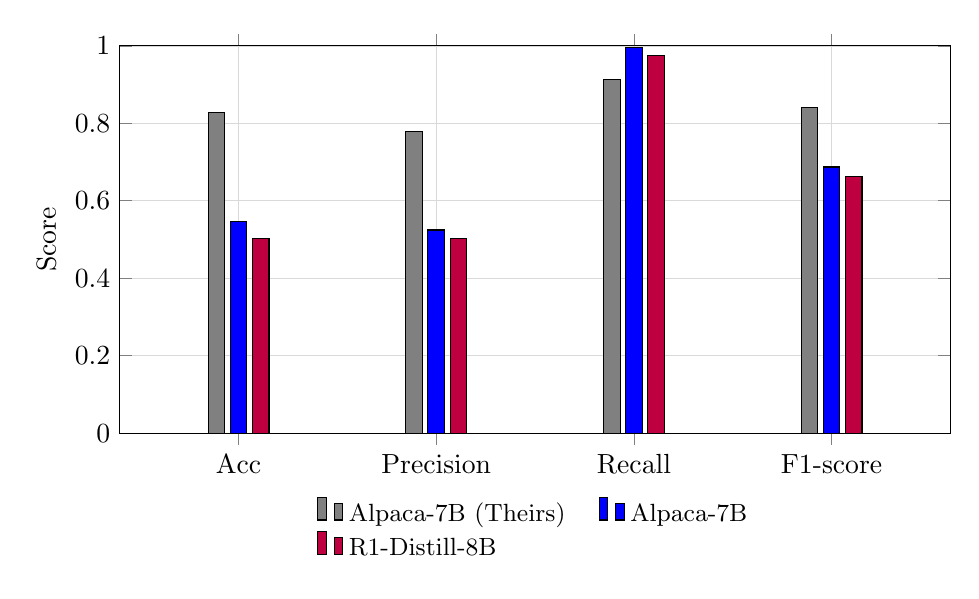
\begin{tikzpicture}
            \begin{axis}[
                ybar, bar width=6pt,
                symbolic x coords={Acc, Precision, Recall, F1-score},
                xtick=data, ymin=0, ymax=1,
                ylabel={Score}, width=\linewidth, height=6.5cm, grid=both,
                major grid style={line width=.2pt, draw=gray!30},
                minor grid style={draw=gray!10},
                enlarge x limits=0.2,
                legend style={
                    at={(0.5,-0.15)}, anchor=north,
                    /tikz/every even column/.append style={column sep=10pt},
                    legend columns=2, draw=none, fill=none,
                    font=\small, nodes={anchor=west}}]

                \addplot[fill=gray]   coordinates {(Acc,0.8274)  (Precision,0.7791)  (Recall,0.9141)  (F1-score,0.8411)};
                \addlegendentry{\modelalpaca (Theirs)}

                \addplot[fill=blue] coordinates {(Acc,0.5465) (Precision,0.5245) (Recall,0.9962) (F1-score,0.6872)};
                \addlegendentry{\modelalpaca}

                \addplot[fill=purple]   coordinates {(Acc,0.5027) (Precision,0.5014) (Recall,0.9759) (F1-score,0.6625)};
                \addlegendentry{\modeldeepseek}

            \end{axis}
        \end{tikzpicture}
    \end{columns}
\end{frame}

%------------------------------------------------

\begin{frame}{KoPA: Fine-tuning}
    \begin{center}
        \begin{tikzpicture}
            \begin{axis}[
                width=0.8\textwidth,
                height=0.8\textheight,
                ymode=log, % Log-scale for better visibility
                xlabel=Epoch,
                ylabel=Loss / Gradient Norm,
                xmin=0, xmax=3, % Consistent x-axis
                ymin=1e-3, ymax=1, % Log scale limits
                xtick distance=0.5,
                ytick distance=10,
                minor y tick num=9,
                grid=major,
                legend style={
                    % at={(1.2, 1)}, % Positioned below
                    anchor=north east,
                    legend columns=1,
                    % draw=none, % No box around legend
                    % fill=none,
                    font=\small,
                    nodes={anchor=west}
                }
            ]

                % Alpaca model
                \addplot[smooth, thick, blue]
                table[x=epoch, y=loss, col sep=space]
                    {../Report/figures/raw-data/lora-Llama-2-7b-alpaca-cleaned-finetune.dat};
                \addlegendentry{\modelalpaca Loss}

                \addplot[smooth, thick, cyan, dashed]
                table[x=epoch, y=grad-norm, col sep=space]
                    {../Report/figures/raw-data/lora-Llama-2-7b-alpaca-cleaned-finetune.dat};
                \addlegendentry{\modelalpaca Grad Norm}

                % DeepSeek model
                \addplot[smooth, thick, purple]
                table[x=epoch, y=loss, col sep=space]
                    {../Report/figures/raw-data/lora-DeepSeek-R1-Distill-Llama-8B-finetune.dat};
                \addlegendentry{\modeldeepseek Loss}

                \addplot[smooth, thick, violet, dashed]
                table[x=epoch, y=grad-norm, col sep=space]
                    {../Report/figures/raw-data/lora-DeepSeek-R1-Distill-Llama-8B-finetune.dat};
                \addlegendentry{\modeldeepseek Grad Norm}

            \end{axis}
        \end{tikzpicture}
    \end{center}
\end{frame}

%------------------------------------------------


\begin{frame}{Conclusion}

    \begin{columns}[t]
        \column{0.40\textwidth}
        \textbf{Results}
        \begin{itemize}
            \item Replicating results is hard
            \item No magic gains from reasoning:
            Also requires engineering to get right
            \item Ideal approach would probably be hybrid
        \end{itemize}

        \column{0.55\textwidth}
        \textbf{KICGPT}
        \begin{itemize}
            \item Fast deployment (no fine-tuning required)
            \item Performance depends on LLM
            \item Results may vary across models
        \end{itemize}
        \textbf{KoPA}
        \begin{itemize}
            \item Fine-tuning leverages KG structure
            \item Requires more computational resources
            \item Needs tuning to balance text and structure
        \end{itemize}
    \end{columns}
    \vspace{4mm}
    \begin{center}
        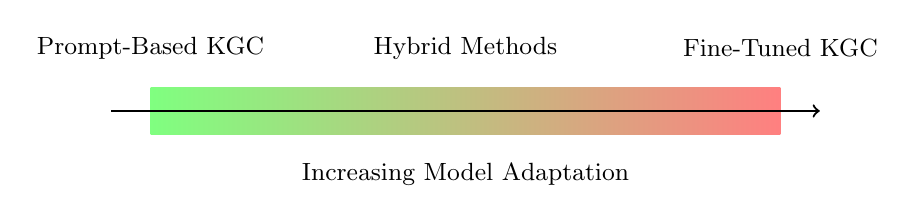
\begin{tikzpicture}
            % Gradient Bar
            \shade[left color=green!50, right color=red!50] (0,-0.3) rectangle (8,0.3);

            % Labels at Start, Middle, and End
            \node[align=center] at (0,0.8) {\small Prompt-Based KGC};
            \node[align=center] at (4,0.8) {\small Hybrid Methods};
            \node[align=center] at (8,0.8) {\small Fine-Tuned KGC};

            % Arrow Showing Spectrum Progression
            \draw[thick,->] (-0.5,0) -- (8.5,0);
            \node[align=center] at (4,-0.8) {\small Increasing Model Adaptation};
        \end{tikzpicture}
    \end{center}
\end{frame}

%\begin{frame}{References}
%    \footnotesize
%    \bibliography{../Report/main}
%    \bibliographystyle{apalike}
%\end{frame}

\backupbegin
%------------------------------------------------
\begin{frame}{Datasets \& Models}
    \begin{columns}[c]
        \column{.45\textwidth}
        Datasets: WN18RR and CoDeX-S.
        \begin{table}[h]
            \centering
            \begin{tabular}{l c c c c c}
                \toprule
                \textbf{Dataset} & \textbf{\# Entities} & \textbf{\# Relations} \\
                \midrule
                WN18RR           & 40,943               & 11                    \\
                CoDeX-S          & 2,034                & 42                    \\
                \bottomrule
            \end{tabular}
            \caption{Statistics of the datasets used in our experiments.}
            \label{tab:datasets}
        \end{table}

        \column{.45\textwidth}
        LLMs Compared:
        \begin{itemize}
            \item \textbf{\modelalpaca} – Fine-tuned for \textit{instruction-following} tasks.
            \item \textbf{\modelministral} – Optimized for \textit{multilingual and long-context} scenarios.
            \item \textbf{\modeldeepseek} – A distilled model with strong \textit{reasoning} capabilities.
        \end{itemize}
    \end{columns}
\end{frame}

\begin{frame}{KoPA: Fine-tuning}
    \begin{figure}
        \centering
        \begin{tikzpicture}
            % Group plot configuration
            \begin{groupplot}[
                group style={
                    group size=3 by 1,       % 3 plots in 1 row
                    horizontal sep=0.3cm     % Adjust spacing between plots
                },
                width=0.3\textwidth,         % Maximized plot width
                ymode=log,                   % Log-scale y-axis for ALL plots
                xmin=0, xmax=3,              % Unified x-axis range
                ymin=1e-3, ymax=1,           % Unified y-axis range across all plots
                xlabel=Epoch,
                xtick distance=0.5,          % Uniform tick spacing
                ytick distance=10,           % Log-scale tick separation
                minor y tick num=9,          % Minor tick marks for readability
            ]

                %------------- Plot (a) Alpaca -----------------
                \nextgroupplot[
                    title=\modelalpaca,
                % Hide y-axis labels for alignment
                    ylabel=Loss
                ]
                \addplot[smooth, thick, blue]
                table[x=epoch, y=loss, col sep=space]
                    {../Report/figures/raw-data/lora-Llama-2-7b-alpaca-cleaned-finetune.dat};

                \addplot[smooth, thick, cyan, dashed]
                table[x=epoch, y=grad-norm, col sep=space]
                    {../Report/figures/raw-data/lora-Llama-2-7b-alpaca-cleaned-finetune.dat};


                %------------- Plot (b) DeepSeek ---------------
                \nextgroupplot[
                    title=\modeldeepseek,
                    yticklabels={,,}
                ]
                \addplot[smooth, thick, purple]
                table[x=epoch, y=loss, col sep=space]
                    {../Report/figures/raw-data/lora-DeepSeek-R1-Distill-Llama-8B-finetune.dat};

                \addplot[smooth, thick, violet, dashed]
                table[x=epoch, y=grad-norm, col sep=space]
                    {../Report/figures/raw-data/lora-DeepSeek-R1-Distill-Llama-8B-finetune.dat};

                %------------- Plot (c) Loss Comparison -------------
                \nextgroupplot[
                    title=Loss Comparison,
                    yticklabels={,,}   % Hide y-axis tick labels for uniform look
                ]
                \addplot[smooth, thick, purple]
                table[x=epoch, y=loss, col sep=space]
                    {../Report/figures/raw-data/lora-DeepSeek-R1-Distill-Llama-8B-finetune.dat};

                \addplot[smooth, thick, blue]
                table[x=epoch, y=loss, col sep=space]
                    {../Report/figures/raw-data/lora-Llama-2-7b-alpaca-cleaned-finetune.dat};

            \end{groupplot}
        \end{tikzpicture}

        % Description of colors with more spacing in legend
        \vspace{0.2cm}
        {\centering
            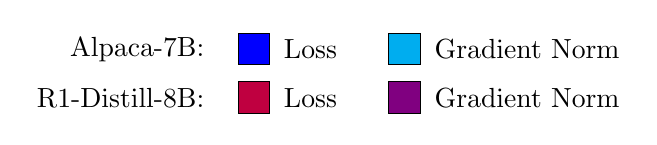
\begin{tikzpicture}
                \node[draw, fill=blue, minimum width=0.4cm, minimum height=0.4cm] (A) {};
                \node[left=0.3cm of A] {\modelalpaca:};
                \node[right=0.05cm of A] {Loss};

                \node[draw, fill=cyan, minimum width=0.4cm, minimum height=0.4cm, right=1.5cm of A] (B) {};
                \node[right=0.05cm of B] {Gradient Norm};

                \node[draw, fill=purple, minimum width=0.4cm, minimum height=0.4cm, below=0.2cm of A] (C) {};
                \node[left=0.3cm of C] {\modeldeepseek:};
                \node[right=0.05cm of C] {Loss};

                \node[draw, fill=violet, minimum width=0.4cm, minimum height=0.4cm, right=1.5cm of C] (D) {};
                \node[right=0.05cm of D] {Gradient Norm};
            \end{tikzpicture}
        }

        \caption{Fine-tuning of \modelalpaca and \modeldeepseek. Loss and gradient norm trends are shown separately for each model, along with a comparison of both losses. Figure and results from our work.}
        \label{fig:training_comparison}
    \end{figure}
\end{frame}
\backupend

\end{document}
